\documentclass{article}
\usepackage{setspace}
\doublespacing
\usepackage[utf8]{inputenc}
\usepackage{color}
\usepackage{bm,amsmath}
\usepackage{graphicx}
%\usepackage{epstopdf}
%\usepackage{centering}
\usepackage{ragged2e} 
%\title{\textbf{Speaker Recognition using Machine Learning: A Study on Efficacy of Gaussian Mixture Models}}
\vspace{-5em}
\title{\textbf{Efficacy of a Gaussian Mixture Model based Speaker Recognition in Machine Learning Framework}}
\author{\textbf{Adhiraj Banerjee}}

%\centering{\Large{4 week report}}
%(SRFP Application No. : ENGS589)

%\date{18 July 2021}

\begin{document}
\vspace{-3em}
\maketitle
\thispagestyle{empty}
%\centering{\textbf{Dr. Siva Ram Krishna Vadali}\\ Senior Principal Scientist \\ Robotics \& Automation Division, CSIR-CMERI Duragpur}
%\centering{August 2021}
\vspace{-3em}
\begin{center}{\textbf{Dr. Siva Ram Krishna Vadali}\\ Senior Principal Scientist \\ Robotics \& Automation Division\\ 
CSIR-Central Mechanical Engineering Research Institute Duragpur\\}
%\vpsace{1em}
%{August 2021}
\end{center}
\vspace{1em}
\begin{center}{\textbf{August 2021}}
\end{center}
\newpage
\tableofcontents
\newpage
\listoffigures
\newpage
\section{\textbf{{Introduction}}}
%The topic for my Internship which was assigned to me by my guide is, \textit{Speaker Recognition or Identification using Machine Learning}. Here, the problem I have to solve is that I have to create a trained model which will be able to recognize the speaker from its voice sample provided to it as its input. 
\textcolor{black}{Speaker Recognition (SR) has numerous applications such as voice biometric, forensics, traitor finding, voice-mail and  tele-banking. Conceptually, SR determines \textcolor{black}{the presence of the active speaker} among a set of registered speakers. %The present work studies available methods for speaker recognition. Further, 
 \textcolor{black}{In view of the applicability of {Machine Learning} framework to a wide variety of classification problems, the present work studies the popular Gaussian Mixture Model (GMM) based ML (GMM-ML) approach as a potential solution for speaker recognition. Voice samples of ten different speakers are recorded and the performance of GMM-ML for SR is analyzed. Further, performance of GMM-ML is also studied for SR when the speech signal is overlaid with additive noise. It is observed that GMM-ML based SR is fairly accurate in distinguishing the correct speaker from the $10$ registered speakers.}}

\section{\textbf{{``Machine Learning'' for Speaker Recognition}}}
% \textit{Machine Learning} is a method which helps systems to learn from the training data so that they can predict the class of the test data given as input, without being explicitly programmed for this purpose. This same method would be applied in the Speaker Recognition System. Using Machine Learning, a model for Speaker Recognition will be trained in such a way that it will be able to identify unique patterns and features from different voice samples and distinguish a voice sample from the rest. This method can be applied by, firstly \textbf{gathering different people's speech samples}, \textbf{extract features from the voice sample} suitable for the classifier, which is \textbf{trained for building a trained model} and finally,\textbf{performing classification for recognition of each Speaker} from its corresponding input voice sample.
 \textcolor{black}{\textit{Machine Learning} (ML) is a mathematical framework which helps systems to learn and train a model with (preferably) large data sets and subsequently predict the category into which a test data may be classified to.} 
%Without being explicitly programmed for this purpose. 
 \textcolor{black}{The present work studies the efficacy of a ML based classification algorithm for Speaker Recognition. Going by principles of ML}, a model for Speaker Recognition \textcolor{black}{is trained such that the model identifies unique patterns (referred as features) from a set of different voice samples (of registered speakers) and distinguish the actual speaker voice sample from the rest. In the present work, a familiar ML algorithm, Gaussian Mixture Model (GMM) based classification, is chosen and its efficacy in accurate speaker recognition is studied.}
% classification 
 %This method can be applied by, firstly {gathering different people's speech samples}, {extract features from the voice sample} suitable for the classifier, which is {trained for building a trained model} and finally,{performing classification for recognition of each Speaker} from its corresponding input voice sample.


\subsection{Gaussian Mixture Model based SR} 
\textcolor{black}{It is known that the Gaussian Mixture Model (GMM) is a 
%statistical 
powerful model used to solve clustering problems.  
%which is 
%formed by 
It is a probabilistic approach by which it approximates the probability distribution of a $M X K$ length data ($ M$ is the number of $ K$ dimensional data vectors) belonging to a class $\lambda$ (of $L$ classes) as a linear combination of $ N$ Gaussian distributions or clusters %the $i^{th}$ %distribution random variable 
with mean vector $\bm \mu$$=$$\{\mu_i\}_{i=1,2,\ldots,N}$ (i.e. order $K$$X$$1$), variance-covariance \textcolor{black}{matrix} %$\bm \Sigma^\prime$$=$
${\bm\Sigma}$ (i.e. order $K$$X$$K$) and $\bm \omega$$=$$\{\omega_i\}_{i=1,2,\ldots,N}$ (i.e. order $M$$X$$N$) as the weights in the linear combination.} \textcolor{black}{In 
%case of 
\textit{Speaker Recognition}, features of speaker's voice sample 
%which are 
are extracted into a feature vector and used as data points for processing to identify the registered speaker. % to compute the likelihood. %in each model till it is maximized. 
Since the feature vector is \textit{multi-dimensional}, %the likelihood 
the probability density function (PDF) 
%also referred as the likelihood, of a given $N$ dimensional feature vector 
of particular class of speaker ($\lambda$) can be expressed as a linear combination of $N$ multivariate Gaussian PDFs as:
\begin{equation}
P(\bm X\vert\lambda) = \sum\limits_{i=1}^N \omega_i \cdot P(\bm X|\bm \mu_i,\bm \Sigma_i)
\label{eq1}
\end{equation}
and,
\begin{equation}
P(\bm X|\bm \mu_i,\bm \Sigma_i) = \prod\limits_{n=1}^M P(\bm x_n|\bm \mu_i,\bm \Sigma_i)
\end{equation}
where, $M$ denotes the number of Gaussian random variables used for $N$ clusters formed from the input vector $\bm X$; \textbf{$\lambda$}, as mentioned earlier, is the class to which a speaker is associated with; $\bm X$ represents the $N$ dimensional training data; and $P(\bm x_n|\bm\mu_i,\bm\Sigma_i)$ is the multivariate Gaussian PDF given by,%for the $i^{th}$ gaussian distribution.
\begin{equation}
P(\bm x_n|\bm\mu_i,\bm\Sigma_i) = \left({{(2\pi)^N\cdot |\bm\Sigma_i|}}\right)^{-0.5}\cdot exp\left({-0.5 (\bm x_n-\bm\mu_i)^T\bm\Sigma_i^{-1}(\bm x_n- \bm \mu_i)}\right).
\end{equation}
}

\textcolor{black}{In the formulation in Equation \ref{eq1}, the probability, also referred as the likelihood, computed from the input data points in vector $X$ is assigned to a particular class corresponding to the speaker's GMM. Herein, the mean vectors ($\bm \mu_i$), variance-covariance matrices ($\bm\Sigma_i$) and weights of each of the gaussian components ($\bm \omega_i$) is updated iteratively till the likelihood for the data points (i.e. feature vectors) is maximized, %, i.e., fit them in each cluster of the model to create the trained Gaussian Model accordingly w.r.t the extracted features. 
thereby creaing a trained model with the extracted features. The maximized likelihood will thus be assigned to the class corresponding to the speaker, in turn creating the the classified GMM for the speaker.} 

\subsubsection{{The E-M Algorithm}} The \textit{E(Expectation)-M(Maximization)} Algorithm is an iterative statistical algorithm which is used to train Gaussian Mixture Models by updating the unknown parameters($\bm\mu_i$,$\bm\Sigma_i$ \& $\bm\omega_i$) till convergence is achieved. In GMMs, the mean vector, the covariance matrix and the weights of each Gaussian component, for obtaining the maximum log-likelihood of datapoints is unknown, which brings the significance of this algorithm. This algorithm is executed in this fashion:
\begin{itemize}
\item \underline{Initialization}: At first, arbitary values are taken for initializing the mean vector($\bm\mu_i$), covariance matrix($\bm\Sigma_i$) and weights($\bm\omega_i$) for each of the N Gaussian Distributions or clusters. From these initialized values, the initial Log-likelihood is calculated.
\item \underline{Estimation}: Each of the weights can be considered as a prior probability for each component among all the $N$ Gaussian Clusters. In this step, for every data point or vector($K$-Dimensional $\bm x$$=$$\{x_n\}_{n=1,2,\ldots,M}$), their responsibilities($\bm\gamma_i(\bm x)$ for every gaussian distribution is determined. Responsibilities of every data point can be calculated as their corresponding \textit{Posterior Probabilities} from the previously initialized parameters of each Gaussian component using \textbf{Bayes' Theorem}:
\begin{equation}
\bm\gamma_i(\bm x) = \frac{\bm\omega_i\mathcal{N}(\bm x|\bm\mu_i,\bm\Sigma_i)}{\sum\limits_{j=1}^N \bm\omega_j\mathcal{N}(\bm x|\bm\mu_j,\bm\Sigma_j)}\,where, \bm\omega_i = \frac{\bm M_i}{\bm M}
\end{equation}
Here, $\bm M_i$ is the effective number of data points assigned to the gaussian cluster $\bm i$ and $\bm M$ is the total number of datapoints for each speaker.
\item \underline{Maximization}: In this step, the parameters of each of the $N$ Gaussian Clusters are re-estimated using the current Responsibilities of each data vector $\bm x$$=$$\{x_n\}_{n=1,2,\ldots,M}$ for a particular Gaussian component. The mathematical form for each of the paramaters of a Gaussian Cluster is given below:
\begin{enumerate}
\item \textbf{Mean Vector($\bm\mu_i$)}:
\begin{equation}
\bm\mu_i = \frac{\sum\limits_{n=1}^M\bm\gamma_i(\bm x_n)\bm x_n}{\sum\limits_{n=1}^M\bm\gamma_i(\bm x_n)}
\end{equation}
\item \textbf{Covariance Matrix($\bm\Sigma_i$)}:
\begin{equation}
\bm\Sigma_i = \frac{\sum\limits_{n=1}^M\bm\gamma_i(\bm x_n)(\bm x_n-\bm\mu_i)(\bm x_n-\bm\mu_i)^T}{\sum\limits_{n=1}^M\bm\gamma_i(\bm x_n)}
\end{equation}
\item \textbf{Weight of each Cluster($\bm\omega_i$)}:
\begin{equation}
\bm\omega_i = \frac{1}{\bm M}\sum\limits_{n=1}^M\bm\gamma_i(\bm x_n)
\end{equation}
\end{enumerate}
\item \underline{Evaluating the Log-Likelihood}: Here, from the estimated parameters of each Gaussian component in the previous step, the Log-Likelihood of the data points belonging to a particular class of speaker $\bm\lambda$ is calculated, as shown below:
\begin{equation}
\ln P(\bm X|\lambda) = \sum\limits_{n=1}^M\ln\sum\limits_{i=1}^N\bm\omega_i\mathcal{N}(\bm x_n|\bm \mu_i,\bm \Sigma_i)
\end{equation}
\end{itemize}
If convergence of data points to the $\bm N$ Gaussian Clusters is not fulfilled, then starting from the second step, all the steps need to be repeated again. The criteria for which convergence has occurred in the E-M Algorithm is as follows:
\begin{enumerate}
\item If the parameters of the Gaussian components($\bm\mu_i,\bm\Sigma_i \,\&\, \bm\omega_i$) does not change in the last successive iterations.
\item If the Log-Likelihood of the data points for a particular speaker remains the same(indicating its maximization) in the last few iterations.
\end{enumerate}
\subsection{Feature Extraction in SR: Mel-Frequency Cepstrum Coefficients(MFCC)}
The features which are extracted from the voice samples, are called, \textit{MFCC (Mel-Frequency Cepstrum Coefficients)}. MFCCs have become a prominent feature to be used for feature extraction from train data, because it gives an idea about the perceived difference between frequencies, especially in higher frequency region. Its importance comes from the fact that, \textit{the human ear can perceive voice signal frequncies non-linearly}. From here, there is a clear understanding that while using Signal-Processing in this case, frequencies needs to be analyzed in the \textit{Mel} scale, rather than the {Hertz} scale. There is logarithmic(non-linear) relationship between the Mel and Hertz scale, from which frequncies in Mel scale becomes more useful. The extraction of MFCCs can be theoretically elaborated in the steps below:
\begin{itemize}
\item \textbf{\underline{Pre-Emphasis}:} At first, Pre-Emphasis(after discretization of the analog voice signal) is done to increase the energy of the signal at higher frequencies, the frequency range where the human ear tends to perceive less in linear scale. Pre-Emphasis is mainly done for transmission cases which brings the significance of prescence of higher frequency components in the voice signal. This process is done by passing the signal through a \textit{First-Order High Pass Filter}. The equation for the signal (x[n]) and its output signal (y[n]) after passing through the filter is below:
\begin{equation}
\bm{y[n]} = \bm{x[n]} - \bm{\alpha x[n-1]} \, \forall\, \bm{\alpha}\in (0.9,1) 
\end{equation}
Thus, the z-transform of the filter will be :
\begin{equation}
\bm{H(z)} = 1-\bm{\alpha z}^{-1}
\end{equation}
\item \textbf{\underline{Framing}:} Due to changes in \textit{Prosody}(features of voice) and \textit{random variations} in the vocal tract, the voice signal is a \textit{non-stationary signal(or, random signal)}. However, within short intervals the voice signal is assumed to be \textit{stationary}, for which this signal is analysed over short time windows. Hence, for analysis of voice features, framing is required, as it divides the whole speech signal into short frames of \textbf{N} samples and the adjacent frames are overlapped by \textbf{M} samples($N\,>\,M$).
\begin{figure}[ht]
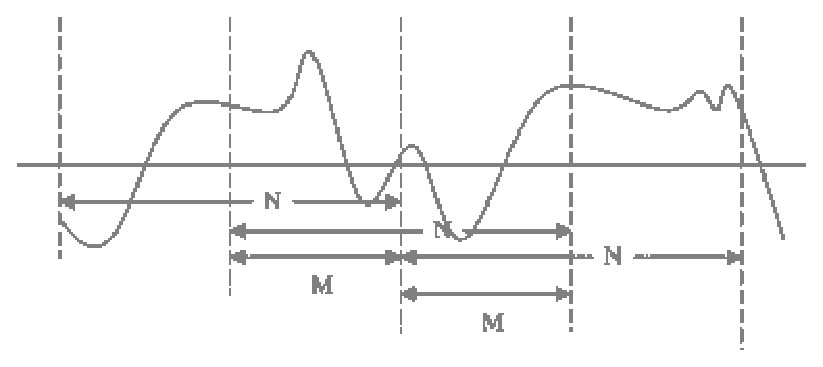
\includegraphics[height=4cm]{fig1.eps}
\centering
\caption{Framing of voice signal}
\label{fig1}
\end{figure}
\item \textbf{\underline{Windowing}:} This process is done to remove discontinuities between frames of the audio signal. When the whole signal is divided into short frames, discontinuities are formed at the edges of the frame, which are incongruent to the input voice signal. These discontinuities may impact the signal by changing the \textbf{Statistical Properties} of the signal. In order to avoid this problem, windowing is executed by multiplying each frame with a window, a smooth function which goes zero at the borders. Generally, the signal frames are multiplied with the \textit{Hamming Window}. Considering the window to be w[n], the equation for windowing is :
\begin{equation}
y[n] = x[n]\cdot w[n]
\end{equation}
where, $\bm{x[n]}$ is the Input Signal, $\bm{y[n]}$ is the Output Signal and for N being the number of samples in each frame,
\begin{equation}
\bm{w[n]} = 0.54-0.46\cdot\bm{\cos{\frac{2\pi n}{N-1}}}\,\forall\,\bm{n\,\in\,[0,N-1]}
\end{equation}
\item \textbf{\underline{Performing the FFT(Fast Fourier Transform)}:}We need to execute the \textit{FFT or $N_1$-point DFT (Discrete Fourier Transform)} of each frame of the signal to obtain their frequency spectrum from the absolute value of the DFT(time domain to frequency domain). $N_1$ should be greater than the total sample size of each frame. The spectrum plot is considered from k = 0,.....,$\frac{N_1}{2}$, where $f_{Hz} = k\frac{f_s}{N_1}$, $f_s$ being the sampling frequency and $k\frac{f_s}{N_1}$ is called Resolution. The formula for the FFT can be expressed as:
\begin{equation}
\bm{X[k]} = \sum\limits_{n=0}^{N_1-1}\bm{x[n]\cdot \exp{\frac{-j2\pi nk}{N_1}}}\,\forall\, \bm{k}=0,1,.....,\bm{\frac{N_1}{2}}
\end{equation}
where, $\bm{x[n]}$ is the input signal(or, short frame) and $\bm{X[k]}$ is the FFT of the input x[n]. Here, $\bm{|X[k]|}$ gives the frequency spectrum of the frames of the input voice signal.
\item \textbf{\underline{Mel-Filter Bank Processing}:} The frequency spectrum is then passed through a Mel-filter bank, which is a bank of triangular filters plotted against frequencies in Mel Scale. The relationship between frequencies in Hz scale and frequencies in Mel-scale can be expressed as:
\begin{equation}
\bm{f}_{Mel} = 2595\log{(1\,+\,\frac{\bm{f}_{Hz}}{700})}
\end{equation} 
\begin{figure}[ht]
\centering

\includegraphics[width=17cm,height=7cm]{fig2.eps}
\caption{Relationship between Mel-scale and Hz-scale}
\end{figure}
%Here, $L$ filters are used within $k$ = $0,...,$$\frac{N}{2}$. 

The filter output we get after passing the frequency spectrum into Mel-filter bank gives the Mel-Frequency Spectrum. The equation for the filter output $\tilde S(l)$ is given below:
\begin{equation}
\bm{\tilde S(l)} = \sum\limits_{k=0}^{N_1/2}\bm{S(k)\cdot M_l(k)}\,\forall\,\,\bm{l} = 0,1,.....,\bm{L}-1
\end{equation}
where, $\bm{S(k)=|X[k]|}$ is the Frequency Spectrum for the input $\bm{x[n]}$ and $\bm{L}$ is the number of Triangular Mel-filters used for filtering the whole spectrum to obtain the Mel-frequency spectrum over the whole range of $k$.
The spectrum obtained from filtering operation renders non-linear frequency spectrum at the higher frequencies.% which human ear can obtain. This way, though the bandwidth is kept same, the perceived difference between frequencies can also be obtained in all frequency ranges. 
The Mel-filter bank usage is important as Voice signal generally follows frequencies in non-linear form and thus the human ear can perceive frequencies being non-linear.
\begin{figure}[ht]
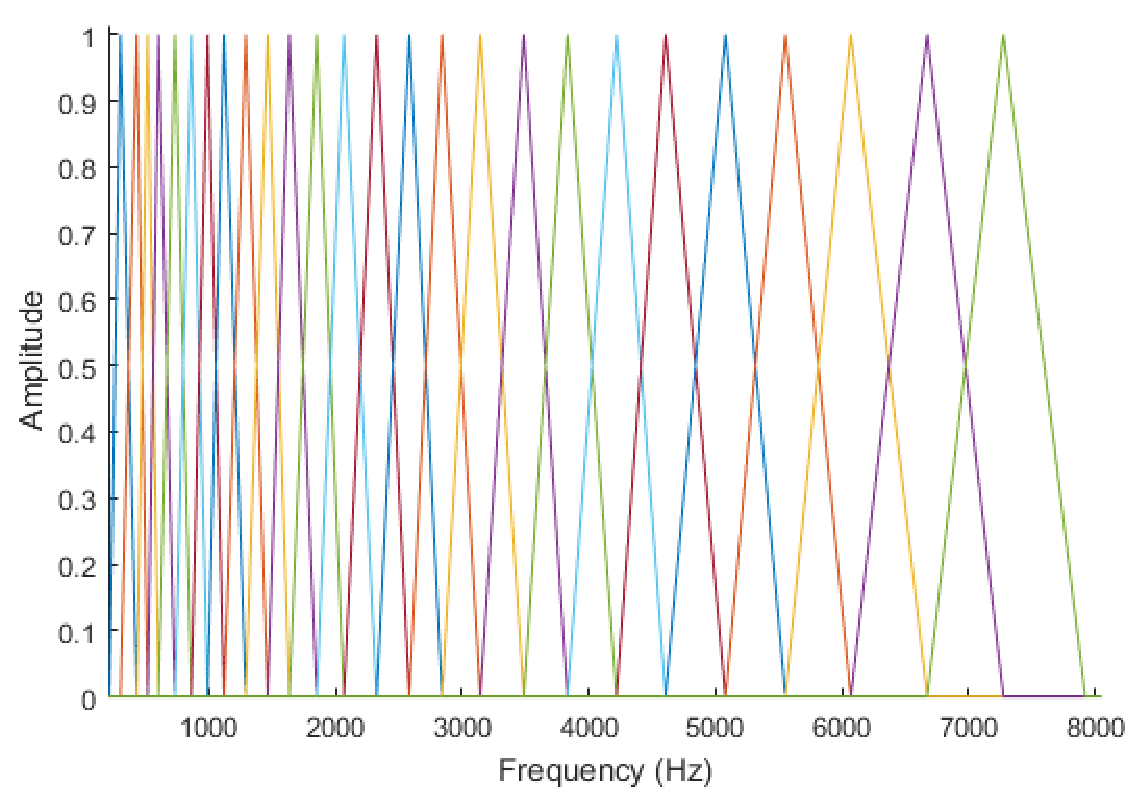
\includegraphics[width=14cm,height=6cm]{fig3.eps}
\caption{Triangular Mel-Filter Bank}
\centering
\label{fig2}
\end{figure}
\item \textbf{\underline{Conversion of Mel- Spectrum to Mel-Cepstrum}:} The logarithm of the Mel-frequency spectrum is taken to obtain Mel-Frequency Cepstrum.
\begin{figure}[ht]
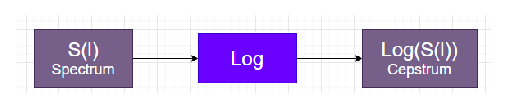
\includegraphics[width=14cm,height=2cm]{fig4.eps}
\caption{Conversion of Spectrum to Cepstrum}
\centering
\label{fig3}
\end{figure}
\item \textbf{\underline{Obtaining the MFCCs}:} The Cepstrum obtained in previous step, is operated upon by taking its \textit{Discrete Cosine Transform(DCT)} which provides us MFCCs as the final result. The equation for the performed DCT is as follows:
\begin{equation}
\bm{c(i)} = \sqrt{\frac{2}{L}}\sum\limits_{m=1}^L\bm{\log{(\tilde S(m))}\cdot \cos{(\frac{\pi i}{L}(m-0.5))}}\,\forall\,\bm{c}=0,1,.....,\bm{C}-1
\end{equation}
where, $\bm{C}$ is number of MFCCs desired, $\bm{\log{(\tilde S(m))}}$ is the Mel-Cepstrum obtained and $\bm{L}$ is the number of triangular mel-filters used for obtaining the Mel-Spectrum.
\end{itemize}
\section{\textbf{Observations in accuracy of GMM in SR for Speech samples with noise}}
In the above sections, it has been discussed that how from the speech samples provided, the features are extraced from the training files using which the Gaussian Mixture Models(GMM) are trained. It has been observed that, for the speech samples which had been recorded and stored for training and testing purposes have given good results( 100\% approx. ).

In practical situations, noise from the surrounding areas are of random nature and may distort the statistical properties of the voice signal. Hence, in order to test the efficiency of GMM for speaker recognition, for a particular class of speaker, GMMs have been trained after applying additional Gaussian Noises with different variances to the audio extracted from the training files, and the accuracy had been tested for a case of noise of particular variance. The Noise Variance versus Accuracy table is given below:
\begin{table}[h]
\centering
\begin{tabular}{|c|c|}
\hline
\multicolumn{1}{|l|}{Variance of Noise} & \multicolumn{1}{l|}{Accuracy(in \%)} \\ \hline
$10^{-10}$               & 100                                 \\ \hline
$10^{-8}$                & 92.59                               \\ \hline
$10^{-6}$                & 81.48                               \\ \hline
$10^{-5}$                & 59.25                               \\ \hline
$10^{-4}$                & 37.03                               \\ \hline
$10^{-2}$                & 22.22                               \\ \hline
$1$                       & 7.407                              \\ \hline
\end{tabular}
\end{table}

The above table gives an idea about the efficiency of GMM in Speaker Recognition system. It is acknowledged that for adding noises with variance above $10^{-5}$ the accuracy of detection goes below $50\%$ which can be explained on the basis of the \textbf{Signal-to-Noise Ratio}(i.e., SNR). The approximate power for each of the audio samples used for training phase was observed in python and minimum of them was seen to be just above $10^{-4}$. As a result of this, for some speakers the noise with variances above $10^{-5}$ could distort the audio samples and the GMMs could not be trained properly. Due to this, speaker recognition for some of the speech samples in testing phase could not function, thus, leading to accuracy decreasing below $50\%$.
\begin{figure}[ht]
\includegraphics[width=19cm,height=10cm]{audio.eps}
\caption{Audio Signals with \& without noise}
\label{fig5}
\end{figure}


The Gaussian Noise has been added to the audio samples of each speaker by creating noise using \textit{numpy.random.normal}(mean,std\_dev,audio) in python. If it is considered that $\bm y$ is the output signal with $\bm x$ as the input signal and $\bm n$ as the additional Gaussian noise, then:
\begin{equation}
\bm y = \bm x + \bm n
\end{equation} 

\section{\textbf{{Results and Inference}}} \label{result}
\textcolor{black}{In the present work, 
%From the results after testing the related python codes, 
GMM based Speaker Recognition is tested for its efficacy over $10$ speakers. The entire coding is done in a Python environment. It is observed that GMM based SR is highly accurate (100$\%$ approx).%, if the approach of \textbf{GMM-ML} for \textbf{Speaker Recognition} is used. 
Hence, it can be inferred that this approach for accomplishing Speaker Recognition(SR) is highly efficient and can be used in practical applications where SR is important.}

\section{\textbf{{Conclusion on Work Done}}}
%I would like to conclude this report by stating that, the 
Speech Recognition is a \textit{text-dependent} method, where it highly depends on the language and corpus. \textcolor{black}{On the other hand, Speaker Recognition mainly focusses on raw audio percepts (and from the information derived therein) %by which it identifies the 
to identify the uniqueness aspect, if any, among different speakers. \textit{Machine Learning} is a holistic approach which renders \textit{Speaker} Recognition efficient when compared to \textit{Speech} Recognition methods for Speaker idenfitication applications. %Hence, \textbf{Machine Learning} helps us to achieve the goal of Speaker Recognition and makes us understand about differences between \textit{Speaker Recognition} \& \textit{Speech Recognition}.
%As discussed in section \ref{result}, the results which are obtained when the python codes are executed, are observed to be quite accurate, which concludes that the \textit{GMM-ML} approach can be a highly efficient solution for achieving \textit{Speaker Recognition }(SR) practically.
In this work, performance of GMM-ML is studied for classifying active speaker identification problem, for both clean speech and speech corrupted with additive Gaussian noise. \textcolor{black}{It is found that $100\%$ accuracy may be achieved when tested over 10 different speakers.}}
\end{document}